%
% Manual for Healthstone - (C) 2015 Patrick Lambert
% Compile with XeLaTeX
%

% Document class
\documentclass[11pt]{article}
\usepackage{geometry}
\usepackage{listings}

% Margins and paper type
\geometry{a4paper, right=1.5cm, left=1.5cm, top=2cm, bottom=1.5cm}

% Color definitions
\usepackage{color}
\usepackage{hyperref}
\definecolor{headings}{rgb}{0.84,0,0.53}
\hypersetup{colorlinks, linkcolor={red}, citecolor={red}, urlcolor={red}}

% Paragraph indent and spacing
\usepackage[english]{babel}
\setlength{\parindent}{0em}
\setlength{\parskip}{1em}
\usepackage{indentfirst}
\usepackage{setspace}

% Section titles
\usepackage{titlesec}
\titleformat{\section}
{\color{headings}\normalfont\LARGE\bfseries}
{\color{headings}\thesection}{1em}{}
\titleformat{\subsection}
{\color{headings}\normalfont\Large\bfseries}
{\color{headings}\thesubsection}{1em}{}
\titleformat{\subsubsection}
{\color{headings}\normalfont\large\bfseries}
{\color{headings}\thesubsubsection}{1em}{}

% Font definition
\usepackage{fontspec}
\setmainfont{Arial}

% Header setup
\usepackage{fancyhdr}
\pagestyle{fancy}
\fancyhf{}
\rhead{\large{\textsc{\color{headings}{\thepage}}}}
\lhead{\large{\textsc{\color{headings}{Healthstone Monitoring System}}}}

% Document starts
\begin{document}

\begin{titlepage}
\bigskip
\begin{center}
\begin{figure}
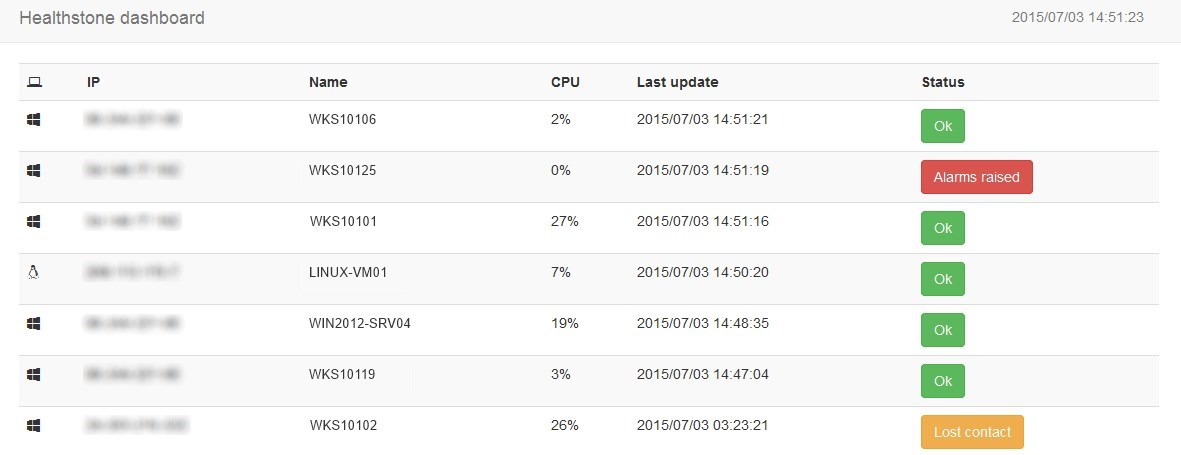
\includegraphics[scale=0.6]{splash.jpg}
\end{figure}
\vspace*{1cm}
{\setstretch{5.0}
{\Huge \color{headings}{Healthstone Monitoring System}}\\
\bigskip
{\Large Patrick Lambert}\\
\texttt{\url{http://healthstone.ca}}\\
\bigskip
v1.2.2}
\vspace*{\fill}
\end{center}
\end{titlepage}

\tableofcontents

\newpage

\section{Introduction}

Healthstone is an open source and lightweight system monitoring solution able to run dozens of customizable health checks. The client component runs as a Windows service or Linux cron job and can notify the Event Log, send emails, file a NodePoint ticket, run a custom program, or send a notification using Amazon SNS or Pushbullet in case any health check fails. It runs on any 64 bits Windows XP, 7, 8, 10, Server 2008 or Server 2012 system, or a Linux system. It can be used to monitor servers or the state of Windows desktops in any environment, along with other services such as IIS, SQL Server, etc. It also includes a server component which provides an optional dashboard against which the Healthstone clients can register.

A typical scenario would be to have a number of Windows desktops in a LAN configuration. For this, you can easily place the Windows client files on a central network location, and run the installation through Group Policy. You may also have some Linux and Windows servers spread through various datacenters and cloud locations, where you can manually install clients. Finally, you can select one server to run the dashboard, against which all of your clients will register, and where you can monitor the health of your whole network from a central location.

You may configure each client to have the ability to send you notifications through a number of means, or have them only report to the dashboard, and have your dashboard report to you if any of the clients raised alarms.

\section{Windows client}

The Healthstone Windows client is a small binary along with a configuration file. The binary runs as a Windows service and checks the current system for all configured health checks on a regular interval. This service is only a few KBs in size and takes a few MBs of system memory to run. On startup, it reads the configuration file from a standard location at \texttt{C:\textbackslash Program Files\textbackslash healthstone\textbackslash healthstone.cfg} and follows those settings until stopped. Note that you can modify the location of this file by changing the Registry key \texttt{HKLM/SOFTWARE/Healthstone}. This can be useful if you wish to use a single config file for all your Windows systems, accessible on a mapped drive.

When the Windows service notices a health check failed (or even on success, should you configure it that way), a number of notifications can be sent. This can include email notifications, creating a NodePoint ticket, sending a PushBullet notification to your phone, or notifying a Healthstone dashboard. Note that this package is all you need to monitor a Windows system, but the dashboard component is a useful companion to run if you wish to keep track of multiple systems.

Along with the service file and configuration file, an installation batch script is provided, and this document.

\subsection{Installation}

The client component can run on any 64 bits Windows host and requires Microsoft .NET Framework 4.5 to be installed.

\begin{enumerate}
\item Download ans extract \texttt{healthstone-client-win64.zip} onto each host you want to monitor, or to a central accessible network location.
\item Edit \texttt{healthstone.cfg} and customize the checks you want to run.
\item Run \texttt{install.bat} as a local administrator on each host to copy the files and install the service.
\end{enumerate}

The install file will go through several steps. First, it will copy the binary and configuration files to\\ \texttt{\%PROGRAMFILES\%\textbackslash healthstone}. Then, it will add the location of the configuration file to the Registry. Finally, it will create and start the Windows service.

\subsection{Troubleshooting}

You can look at the Event Log to see whether the service started correctly, and if any error occurred. At every interval, a new entry will be added with a result of the health checks. Note that all of the configuration file entries must be present, do not remove any line. If the service fails to start, an error message should be shown in the Event Log. A typical reason may be if the configuration file cannot be found or is corrupted. You can also try to manually run the binary file to see whether it launches. This can be useful to know if you're missing the .NET Framework, for example.

\subsection{Configuration}
Configuration for the Windows service is done in the \texttt{heaslthstone.cfg} file. Note that you will need to restart the service after any change. This file comes with sane default values, but you still should go over all the options to configure them depending on your needs.

\begin{itemize}
\item Interval (in seconds) to run checks. [number]\\
\texttt{Interval: 300}
\item Always raise an alarm, regardless of results. [true|false]\\
\texttt{AlwaysRaise: false}
\item Show full system information, not just failed checks. [true|false]\\
\texttt{Verbose: false}
\item Custom text to add at the end of all reports. [text]\\
\texttt{CustomText:}
\item Raise errors instead of warnings in the Event Log. [true|false]\\
\texttt{RaiseErrors: false}
\item Raise an alarm if a test query fails or is not supported on the system. [true|false]\\
\texttt{RaiseQueryFailures: false}
\item Log debug information about notifications, used to troubleshoot failed notifications. [true|false]\\
\texttt{NotifyDebug: false}
\item Use a proxy server for web based notifications. [url|false]\\
\texttt{NotifyProxy: false}
\item Set to true if you're having issues connecting to SSL servers. [true|false]\\
\texttt{NotifySSL: false}
\item Address of a Healthstone dashboard. [url|false]\\
\texttt{NotifyHealthstoneDashboard: false}
\item File a NodePoint ticket. [true|false]\\
\texttt{NotifyNodePoint: false}
\item NodePoint server address. [url]\\
\texttt{NotifyNodePointAddress: http://10.10.106.2/nodepoint}
\item NodePoint API key. [text]\\
\texttt{NotifyNodePointKey: XXXXXXXXXXXXXX}
\item NodePoint product id. [number]\\
\texttt{NotifyNodePointProduct: 1}
\item Send a Pushbullet notification. [true|false]\\
\texttt{NotifyPushbullet: false}
\item Pushbullet key. [text]\\
\texttt{NotifyPushbulletKey: XXXXXXXXXXXXXX}
\item Send mail notifications. [true|false]\\
\texttt{NotifyEmail: false}
\item SMTP server name. [hostname]\\
\texttt{NotifyEmailServer: smtp.example.com}
\item SMTP server port. [number]\\
\texttt{NotifyEmailPort: 25}
\item SMTP from address. [email]\\
\texttt{NotifyEmailFrom: noreply@example.com}
\item SMTP to addresses. Separate email addresses with spaces. [email email email]\\
\texttt{NotifyEmailTo: tyrion.lannister@example.com}
\item Run custom program. Report content will be passed as command line arguments. [program|false]\\
\texttt{NotifyProgram: false}
\item Send Amazon SNS notification to a topic ARN. [topicarn|false]\\
\texttt{NotifyAWSTopic: false}
\item AWS region where the SNS topic is defined. [region]\\
\texttt{NotifyAWSRegion: us-west-2}
\item AWS IAM access key ID with access to publish to that topic. [key]\\
\texttt{NotifyAWSKey: XXXXXXXXX}
\item AWS IAM secret with access to publish to that topic. [secret]\\
\texttt{NotifyAWSSecret: XXXXXXXXXXXXXXXXXXXXXXX}
\item Check whether Data Execution Prevention is set. [true|false]\\
\texttt{CheckDEP: true}
\item Check for a specific time zone. Number, in hours, the system is offset from Greenwich Mean Time (GMT). Example: PST is -8. [number|false]\\
\texttt{CheckTimeZone: false}
\item Check for a specific code page. Example: Hebrew is 1255. [number|false]\\
\texttt{CheckCodePage: false}
\item Check if free physical memory is lower than x megabytes. [number|false]\\
\texttt{CheckFreeMemory: 200}
\item Check whether the system rebooted in the past x hours [number|false]\\
\texttt{CheckLastBoot: false}
\item Check if the system locale is set to a specific value. Example: EN-US is 0409. [number|false]\\
\texttt{CheckLocale: false}
\item Check overall system status as reported by the Windows subsystem. [true|false]\\
\texttt{CheckSystemStatus: true}
\item Check if there are more than x processes running on the system. [number|false]\\
\texttt{CheckProcessCount: 200}
\item Check if a list of processes are running. Use the binary names, separated with spaces. [process process process|false]\\
\texttt{CheckProcesses: false}
\item Check if an Anti Virus product is installed. Only works on workstations, not servers. [true|false]\\
\texttt{CheckAntiVirus: true}
\item Check if Anti Virus is disabled or out of date. Only works on workstations, not servers. [true|false]\\
\texttt{CheckAntiVirusState: true}
\item Check if the Public firewall is on. [true|false]\\
\texttt{CheckFirewallPublic: true}
\item Check if the Private firewall is on. [true|false]\\
\texttt{CheckFirewallPrivate: true}
\item Check if the Domain firewall is on. [true|false]\\
\texttt{CheckFirewallDomain: true}
\item Check whether the computer booted normally, or in safe mode. [true|false]\\
\texttt{CheckBootState: true}
\item Check whether the machine's DNS hostname is set to a specific value. [text|false]\\
\texttt{CheckHostName: false}
\item Check if the machine is part of a specific domain or workgroup name. [text|false]\\
\texttt{CheckDomainName: false}
\item Check if the CPU temperature is above x degrees Celsius. Does not work with all systems. [number|false]\\
\texttt{CheckTemperature: false}
\item Check if the CPU load is above x\%. [number|false]\\
\texttt{CheckCpuLoad: 90}
\item Check if a specific IP address is reachable using ICMP. [ip|false]\\
\texttt{CheckNetConnectivity: false}
\item Check if the latency with the address in CheckNetConnectivity is above x ms. [number|false]\\
\texttt{CheckNetLatency: 500}
\item Check whether a HTTP URL is working. Will fail if the host is down, page missing, unauthorized, internal server error, etc. [url|false]\\
\texttt{CheckNetHttp: false}
\item Check if an ODBC database connection can be made. Example: Driver={SQL Server};\\ Server=myServerAddress; Database=myDataBase; Uid=myUsername; Pwd=myPassword; [connection string|false]\\
\texttt{CheckODBC: false}
\item Check whether Windows Updates are set to install automatically. [true|false]\\
\texttt{CheckWUEnabled: true}
\item Check if Windows Updates were installed successfully less than x hours ago. [number|false]\\
\texttt{CheckWULast: false}
\item Check if specific Windows Updates are installed. List the Microsoft knowledge base (KB123456) IDs separated with spaces. [kb kb kb|false]\\
\texttt{CheckWUHotFixes: false}
\item Check if any drive has less than x megabytes of space free. [number|false]\\
\texttt{CheckDiskSpace: 500}
\item Check if custom TCP ports are closed on the local system. Separate ports with spaces. [number number number|false]\\
\texttt{CheckCustomPort: false}
\item Check if the time is in sync (<5mins) with this NTP server. [server|false]\\
\texttt{CheckTime: false}
\item Check if a local user exists. [user|false]\\
\texttt{CheckUser: false}
\end{itemize}

\section{Linux client}

The Linux client is a smaller and less fully featured client compared with the Windows client, but should run on a wider array of systems. It supports basic system health monitoring such as whether the host is up, CPU usage, along with a number of notification options.

Like the Windows version, it can be run by itself, configured to notify you when a health check fails. Or, you may pair it with a Healthstone dashboard to have centralized monitoring.

\subsection{Installation}

The client component can run on any Linux host and requires Python 3.x to be installed.

\begin{enumerate}
\item Download and extract \texttt{healthstone-client-linux.tar} onto each host you want to monitor, or to a central accessible network location.
\item Edit \texttt{healthstone.py} and customize the checks you want to run.
\item Run \texttt{sudo ./install.sh} to install the script on the local system.
\end{enumerate}

The installation script will copy the Python file to \texttt{/usr/bin/healthstone.py} and add a crontab entry. This assumes that you can run it as a root. Note that Healthstone can run as a regular user as well. Simply edit the script to copy it to a location you have access to instead. The default crontab is also set to 5 minutes. Modify that time if you're going to change the \textit{Interval} value in the configuration.

\subsection{Troubleshooting}

The install script defaults to adding a 5 minutes crontab for running Healthstone. If you modify the interval value in \texttt{healthstone.py} you should modify that value in the install script as well. You should remove the old crontab entry using \texttt{crontab -e} if you run the install script more than once. Note that being told that \textit{There is no root crontab} is not an error. Finally, if your Python 3.x installation is not in your PATH or at \texttt{/usr/bin/python3} then you may have to edit the crontab.

\subsection{Configuration}

Configuration for the Linux client is done at the top of the \texttt{healthstone.py} file.

\begin{itemize}
\item Interval (in seconds) configured in your crontab between runs [number]\\
\texttt{Interval = 300}
\item Check for acceptable CPU threshold [number|False]\\
\texttt{CheckCPU = 90}
\item Check if a specific process is running [process name|False]\\
\texttt{CheckProcess = False}
\item Check if used disk space is above x percent [number|False]\\
\texttt{CheckDiskSpace = 90}
\item Check if free memory is above x percent [number|False]\\
\texttt{CheckMemory = 90}
\item Check if system rebooted in the last day [True|False]\\
\texttt{CheckReboot = False}
\item Check if a local user exists [user|False]\\
\texttt{CheckUser = False}
\item Check if a URL is returning success or an error [url|False]\\
\texttt{CheckURL = False}
\item Notify a Healthstone dashboard [url|False]\\
\texttt{NotifyDashboardURL = "http://localhost/healthstone"}
\item Write alarms to a log file [filename|False]\\
\texttt{NotifyFile = False}
\item Run a custom shell command when alarms fail [command|False]\\
\texttt{NotifyProgram = False}
\item Send a Pushbullet notification [API key|False]\\
\texttt{NotifyPushbullet = False}
\end{itemize}


\section{Dashboard}

The dashboard is a Python script that runs on an IIS or Apache web server and awaits connections from clients. Once a client connects, it stores the data it receives, and optionally sends a notification if the client reported health check failures or stops checking in. You can connect to the dashboard web site and login using the access code configured inside of the script, then view a table of all the clients that reported in. By clicking on the status icon, you can also view more details about a specific host, such as a graph of past CPU utilization, a history of alarms and lost contact, along with the last check in time.

The dashboard also distinguishes between Linux and Windows hosts, and tracks hosts based on the hostname, not the IP address. This means a single host will keep its entry even if its IP address changes.

\subsection{Installation}

The server component runs the dashboard against which Healthstone clients can register. It is not mandatory, and Healthstone clients can be run without a dashboard. It requires Python 3.x and runs on IIS or Apache with CGI and ISAPI support enabled.

\begin{itemize}
\item Download \texttt{healthstone-server.zip} onto your server and unzip it where you want the files to live, for example \texttt{C:\textbackslash healthstone}.
\item Edit \texttt{dashboard.py} and configure the access code and notification settings you want.
\item Run \texttt{setup.bat} as a local administrator on Windows, or create a virtual site linking to the \texttt{www} folder on Linux, making sure the script has write access to \texttt{../db}.
\end{itemize}

Since the dashboard component runs on both Windows and Linux systems, the installation process may vary based on your particular scenario. On Windows, the \texttt{setup.bat} script should handle most default configurations. It will create a local user to run under and add a virtual server under IIS. On Linux, the script should be placed in a publicly available location. A \texttt{.htaccess} file is provided to configure an Apache web server. All data received from clients is kept in a SQLite database under the \texttt{..\textbackslash db} folder.

\subsection{Troubleshooting}

If you get an error loading the site, make sure the rewrite engine is turned on in your web server configuration, so the web configuration file is read. You may need to edit the \texttt{web.config} (Windows) or \texttt{.htaccess} (Linux) files manually depending on your situation. If your Python 3.x installation path is different, you may need to edit those files, along with the \texttt{dashboard.py} file. If you get a 404 error on IIS, make sure you allow the script in \textit{ISAPI and CGI restrictions} inside of IIS Manager.

\subsection{Configuration}

The dashboard configuration is located at the top of the \texttt{dashboard.py} file. Note that dashboard notifications are triggered if any of the clients that check in fail a health check, or stop checking in.

\begin{itemize}
\item Access code to access the dashboard [string]\\
\texttt{AccessCode = "1234"}
\item Send notifications for systems that lose contacts [True|False]\\
\texttt{NotifyOnLostContact = True}
\item Send notifications for systems that raise alarms [True|False]\\
\texttt{NotifyOnAlarms = True}
\item Send a Pushbullet notification using this API key [API key|False]\\
\texttt{NotifyPushbullet = False}
\item Create a NodePoint ticket using this URL, API key, product and release numbers [url|False]\\
\texttt{NotifyNodePointURL = False}\\
\texttt{NotifyNodePointKey = "XXXXXXX"}\\
\texttt{NotifyNodePointProduct = "1"}\\
\texttt{NotifyNodePointRelease = "1.0"}
\item Send an email notification using this SMTP server, To address, and From address [smtp server|False]\\
\texttt{NotifySMTPServer = False}\\
\texttt{NotifySMTPFrom = "me@example.com"}\\
\texttt{NotifySMTPTo = "you@example.com"}
\end{itemize}

\section{Conclusion}

Healthstone is provided as a free open source solution. The source code is available to be viewed and modified from \url{https://github.com/dendory/Healthstone}. Out of the box, it is able to fully monitor a network of machines and report health status through a number of means. If you need more features, you can easily add them to the code.

Should you have questions or comments, feel free to contact the author at \texttt{dendory@live.ca}.

\section{License}
The MIT License (MIT)

Copyright \textcopyright \thinspace 2014-\the\year \thinspace Patrick Lambert

Permission is hereby granted, free of charge, to any person obtaining a copy
of this software and associated documentation files (the "Software"), to deal
in the Software without restriction, including without limitation the rights
to use, copy, modify, merge, publish, distribute, sublicense, and/or sell
copies of the Software, and to permit persons to whom the Software is
furnished to do so, subject to the following conditions:

The above copyright notice and this permission notice shall be included in
all copies or substantial portions of the Software.

THE SOFTWARE IS PROVIDED "AS IS", WITHOUT WARRANTY OF ANY KIND, EXPRESS OR
IMPLIED, INCLUDING BUT NOT LIMITED TO THE WARRANTIES OF MERCHANTABILITY,
FITNESS FOR A PARTICULAR PURPOSE AND NONINFRINGEMENT. IN NO EVENT SHALL THE
AUTHORS OR COPYRIGHT HOLDERS BE LIABLE FOR ANY CLAIM, DAMAGES OR OTHER
LIABILITY, WHETHER IN AN ACTION OF CONTRACT, TORT OR OTHERWISE, ARISING FROM,
OUT OF OR IN CONNECTION WITH THE SOFTWARE OR THE USE OR OTHER DEALINGS IN
THE SOFTWARE.

\end{document}
